% Diese Datei dient als Testseite für Befehle oder Formeln. 
% Alle hier eingegebenen können direkt am Anfang der Arbeit betrachtet werden.

%\begin{figure}
%\begin{center}
%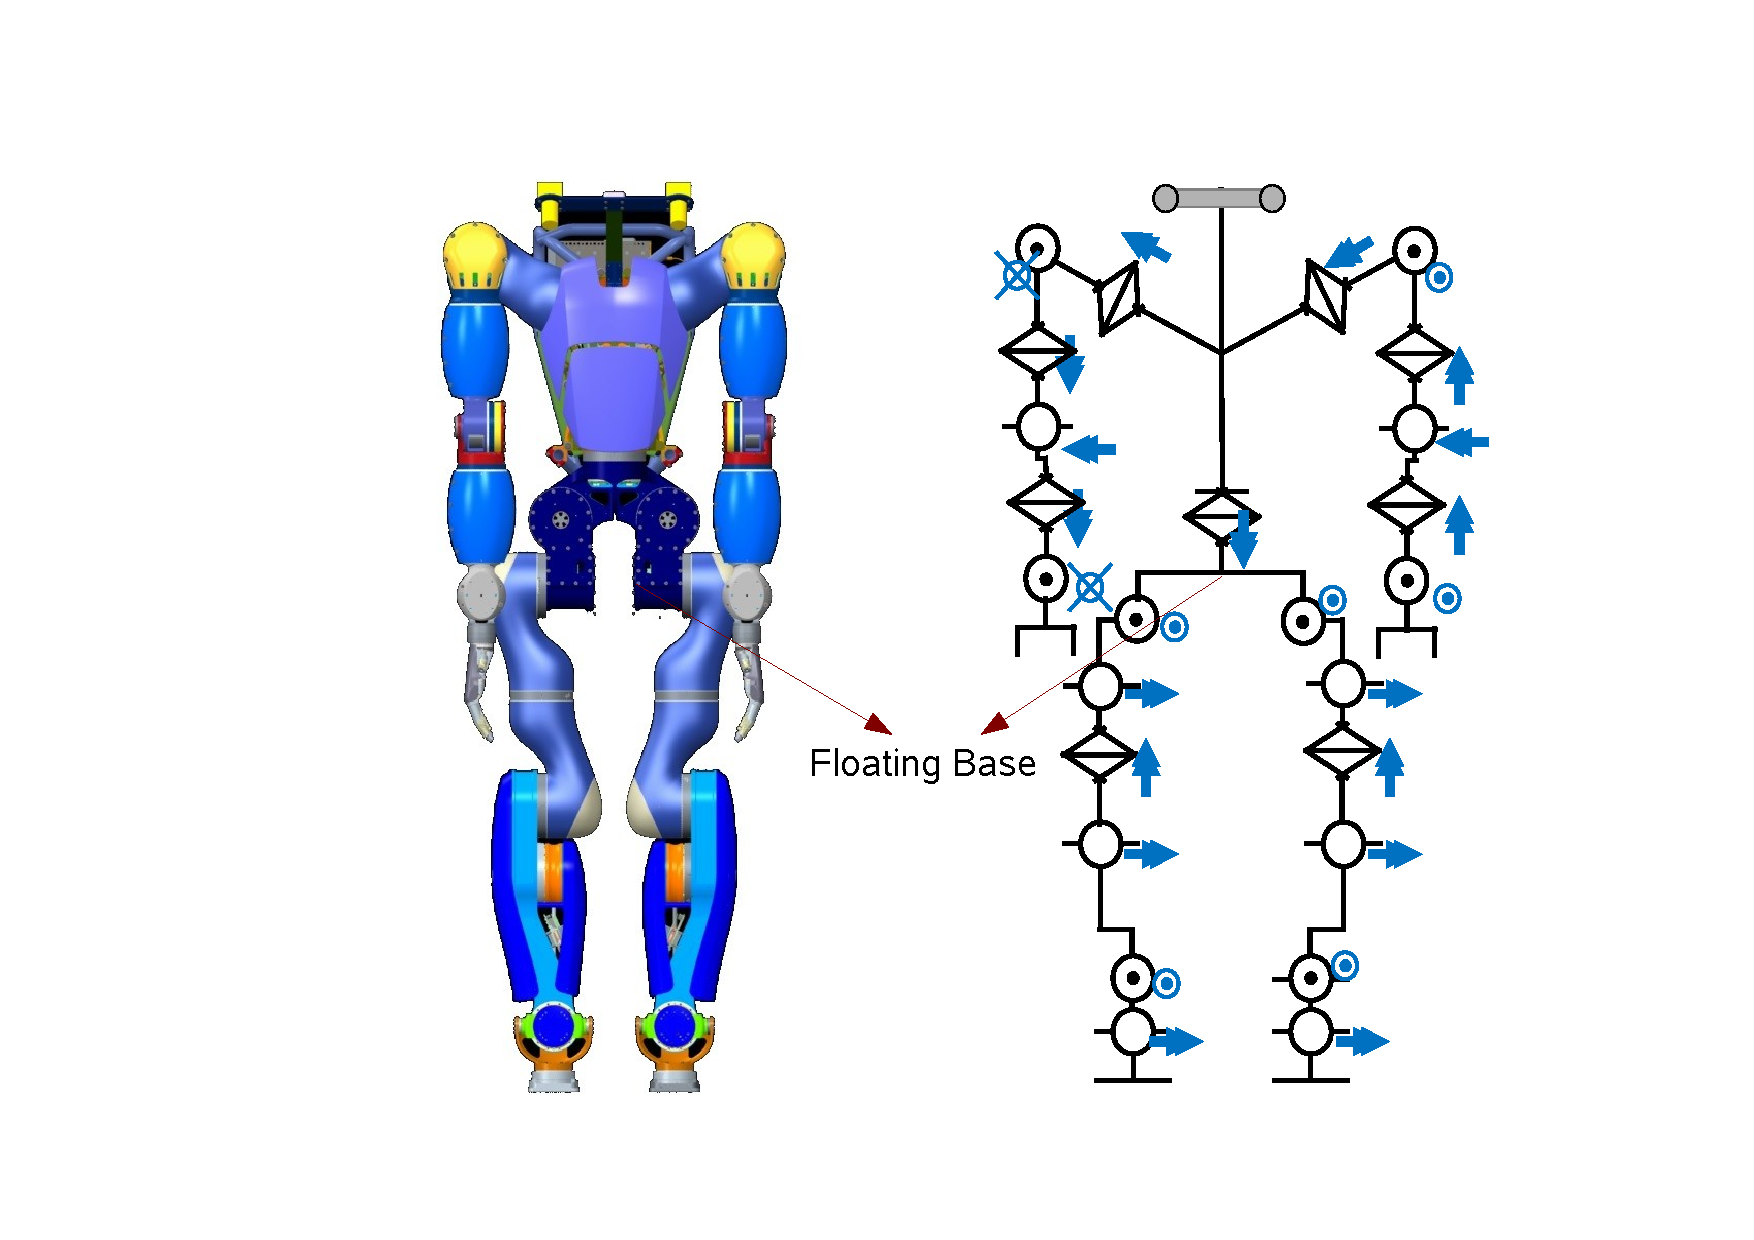
\includegraphics[scale=0.75]{Bilder/TORO_kinematic.pdf}
%\caption{test}
%\label{fig:foo}
%\end{center}
%\end{figure}
\begin{figure}
\tikzstyle{block} = [draw, fill=blue!20, rectangle, 
    minimum height=3em, minimum width=6em]
\tikzstyle{sum} = [draw, fill=blue!20, circle, node distance=1cm]
\tikzstyle{input} = [coordinate]
\tikzstyle{output} = [coordinate]
\tikzstyle{pinstyle} = [pin edge={to-,thin,black}]
\def\blockdist{2.3}
% The block diagram code is probably more verbose than necessary
\begin{tikzpicture}[auto, node distance=4cm,>=latex']
    % We start by placing the blocks
    \node [input, name=input] {};
    \node [sum, right of=input] (sum) {};
    \node [block, right of=sum] (controller) {Controller};
    \node [block, right of=controller, pin={[pinstyle]above:Disturbances},
            node distance=5cm] (system) {System};
    % We draw an edge between the controller and system block to 
    % calculate the coordinate u. We need it to place the measurement block. 
    \draw [->] (controller) -- node[name=u] {$u$} (system);
    \node [output, right of=system] (output) {};
    \node [block, below of= controller] (measurements) {Estimator};

    % Once the nodes are placed, connecting them is easy. 
    \draw [draw,->] (input) -- node {$r$} (sum);
    \draw [->] (sum) -- node {$e$} (controller);
    \draw [->] (system) -- node [name=y] {$y$}(output);
    \draw [->] (y) |- (measurements.base east);
    \draw [->] (u) |- (measurements.10);
    \draw [->] (measurements) -| node[pos=0.99] {$-$} 
        node [near end] {$\hat{x}$} (sum);
\end{tikzpicture}

\caption{Structure of state feedback controller}
\end{figure}